%=======================02-713 LaTeX template, following the 15-210 template==================
%
% You don't need to use LaTeX or this template, but you must turn your homework in as
% a typeset PDF somehow.
%
% How to use:
%    1. Update your information in section "A" below
%    2. Write your answers in section "B" below. Precede answers for all 
%       parts of a question with the command "\question{n}{desc}" where n is
%       the question number and "desc" is a short, one-line description of 
%       the problem. There is no need to restate the problem.
%    3. If a question has multiple parts, precede the answer to part x with the
%       command "\part{x}".
%    4. If a problem asks you to design an algorithm, use the commands
%       \algorithm, \correctness, \runtime to precede your discussion of the 
%       description of the algorithm, its correctness, and its running time, respectively.
%    5. You can include graphics by using the command \includegraphics{FILENAME}
%
\documentclass[11pt]{article}
\usepackage{amsmath,amssymb,amsthm}
\usepackage{graphicx}
\usepackage[margin=1in]{geometry}
\usepackage{fancyhdr}
\usepackage{listings}
\usepackage{float}
\usepackage{subfig}

\setlength{\parindent}{0pt}
\setlength{\parskip}{5pt plus 1pt}
\setlength{\headheight}{13.6pt}
\newcommand\question[2]{\vspace{.25in}\hrule\textbf{#1: #2}\vspace{.5em}\hrule\vspace{.10in}}
\renewcommand\part[1]{\vspace{.10in}\textbf{(#1)}}
\newcommand\algorithm{\vspace{.10in}\textbf{Algorithm: }}
\newcommand\ot{\vspace{.10in}\textbf{Output: }}
\newcommand\runtime{\vspace{.10in}\textbf{Running time: }}
\pagestyle{fancyplain}
\lhead{\textbf{\NAME\ (\ANDREWID)}}
\chead{\textbf{ASS\HWNUM}}
\rhead{\today}
\begin{document}\raggedright
%Section A==============Change the values below to match your information==================
\newcommand\NAME{Yao Xiao}  % your name
\newcommand\ANDREWID{2019180015}     % your andrew id
\newcommand\HWNUM{3}              % the homework number
%Section B==============Put your answers to the questions below here=======================

% no need to restate the problem --- the graders know which problem is which,
% but replacing "The First Problem" with a short phrase will help you remember
% which problem this is when you read over your homeworks to study.

\question{Part1-Step1}{Introduction For MNIST} 
MNIST stands for Mixed National Institute of Standards and Technology, which has produced a handwritten digits dataset. This is one of the most researched datasets in machine learning, and is used to classify handwritten digits. 
This dataset is helpful for predictive analytics because of its sheer size, allowing deep learning to work its magic efficiently. This dataset contains 50000 examples and 784 dimensional feature vecto, formatted as 28 x 28 pixel monochrome images.


\question{Part1-Step2}{Training An SOM}
\textbf{In the process of training SOM, Gaussian distribution and Euclidean distance calculation are used.}

\begin{lstlisting}
class EuclideanDistance {
public:
    float EvaluateDistance(Eigen::VectorXd v1, Eigen::VectorXd v2){
        float KernelValue = (v1 - v2).norm();
        return KernelValue;
    }
};

class GaussianDistribution {
public:
    float Gaussian(float x, float sigma){
        float value = exp(-((float)x/(float)sigma));
        return value;
    }
}
\end{lstlisting}

\textbf{And SOMLearningFunction, UpdateSOMLearningRate, UpdateSOMSigmaNeighbouring are constantly updated during the learning process.}

\begin{lstlisting}
class UpdateSOMLearningRate {
public:
    float UpdateLearningRate(float L0, float LearningRateFinal, float Iter, float lambda){
        float value = (L0 - LearningRateFinal) * L0*exp(-((float)Iter/(float)lambda)) + LearningRateFinal;
        return value;
    }
};


class UpdateSOMSigmaNeighbouring {
public:
    float UpdateSigmaNeighbouring(float SigmaNeighbouringZero, float SigmaNeighbourhoodFinal, float Iter, float lambda){
        float value = (SigmaNeighbouringZero -SigmaNeighbourhoodFinal) * exp(-((float)Iter/(float)lambda)) + SigmaNeighbourhoodFinal;
        return value;
    }
};

\end{lstlisting}

\textbf{The specific training process is as follows:}
\begin{lstlisting}
class SOMTrain :  public Initialize2DMap, public GaussianDistribution,
public SOMLearningFunction, public PrintSOM, public EuclideanDistance, public UpdateSOMLearningRate, public UpdateSOMSigmaNeighbouring, public RandomGenerator {
 public:
 int Iters;
 int BestXMap, BestYMap = 0;
 float Score, ScoreNow = 0;
    float LearningRateInitial, LearningRateFinal, SigmaNeighbouringInitial, SigmaNeighbourhoodFinal, SigmaNeighbouring, LearningRate, lambda;
     
 void Train(int Iters){
     // Initialize alpha
     SOMTrain::SigmaNeighbouringInitial;
     SOMTrain::SigmaNeighbourhoodFinal;
     SOMTrain::LearningRateInitial;
     SOMTrain::LearningRateFinal;
     SOMTrain::LearningRate=SOMTrain::LearningRateInitial;
     SOMTrain::SigmaNeighbouring=SOMTrain::SigmaNeighbouringInitial;
     std::cout <<  SOMTrain::SigmaNeighbouring <<std::endl;
     SOMTrain::lambda = (float)(Iters)/(float)(SOMTrain::xsize/2);
     
     Eigen::VectorXd BMU;
     
     for (int i=0; i<Iters; i++){
         int j = GenerateRandomNumber(SOMTrain::NumberInputVectors);
            // Find the BMU
             for (int RowMap=0;RowMap<SOMTrain::xsize;RowMap++){
                 for (int ColMap=0;ColMap<ysize;ColMap++){
                     ScoreNow = EvaluateDistance(Initialize2DMap::SOMMap(RowMap,ColMap), InputVectors(j,0)); //XX ,1.0 sigma
                     if (ScoreNow > SOMTrain::Score){SOMTrain::Score = ScoreNow; SOMTrain::BestXMap=RowMap, SOMTrain::BestYMap=ColMap;}
                  }
             }
             BMU = Initialize2DMap::SOMMap(SOMTrain::BestXMap,SOMTrain::BestYMap);

             for (int RowMap=0;RowMap<SOMTrain::xsize;RowMap++){
                 for (int ColMap=0;ColMap<ysize;ColMap++){
                     
                     
                     int CoordX = RowMap;
                     int CoordY = ColMap;
                     if (CoordX >= (SOMTrain::xsize/2)){CoordX = (SOMTrain::xsize/2) - RowMap%(SOMTrain::xsize/2);}
                     if (CoordY >= (SOMTrain::ysize/2)){CoordY = (SOMTrain::ysize/2) - ColMap%(SOMTrain::xsize/2);}

                     Eigen::VectorXd BMUUpdated = LearnFunction(Initialize2DMap::SOMMap(RowMap,ColMap),InputVectors(j,0),
                     SOMTrain::BestXMap, SOMTrain::BestYMap, CoordX, CoordY, SOMTrain::SigmaNeighbouring, SOMTrain::LearningRate);
                     Initialize2DMap::SOMMap(RowMap,ColMap) = BMUUpdated;

                 }
             }

         SOMTrain::LearningRate = UpdateLearningRate(SOMTrain::LearningRateInitial,SOMTrain::LearningRateFinal, i, SOMTrain::lambda);
         SOMTrain::SigmaNeighbouring = UpdateSigmaNeighbouring(SOMTrain::SigmaNeighbouringInitial,SOMTrain::SigmaNeighbourhoodFinal,  i, SOMTrain::lambda);
         
         
 }
}
\end{lstlisting}


\question{Part1-Step3}{Parameter Adjustment}
Through continuous experiment adjustment, the initial value of 2D lattices is finally adjusted to 80 X 80, while continuously adjusting NeighbouringInitial, NeighbouringFinal, and learningrate, the experimental process is as follows:

\begin{figure}[H]
    \centering
    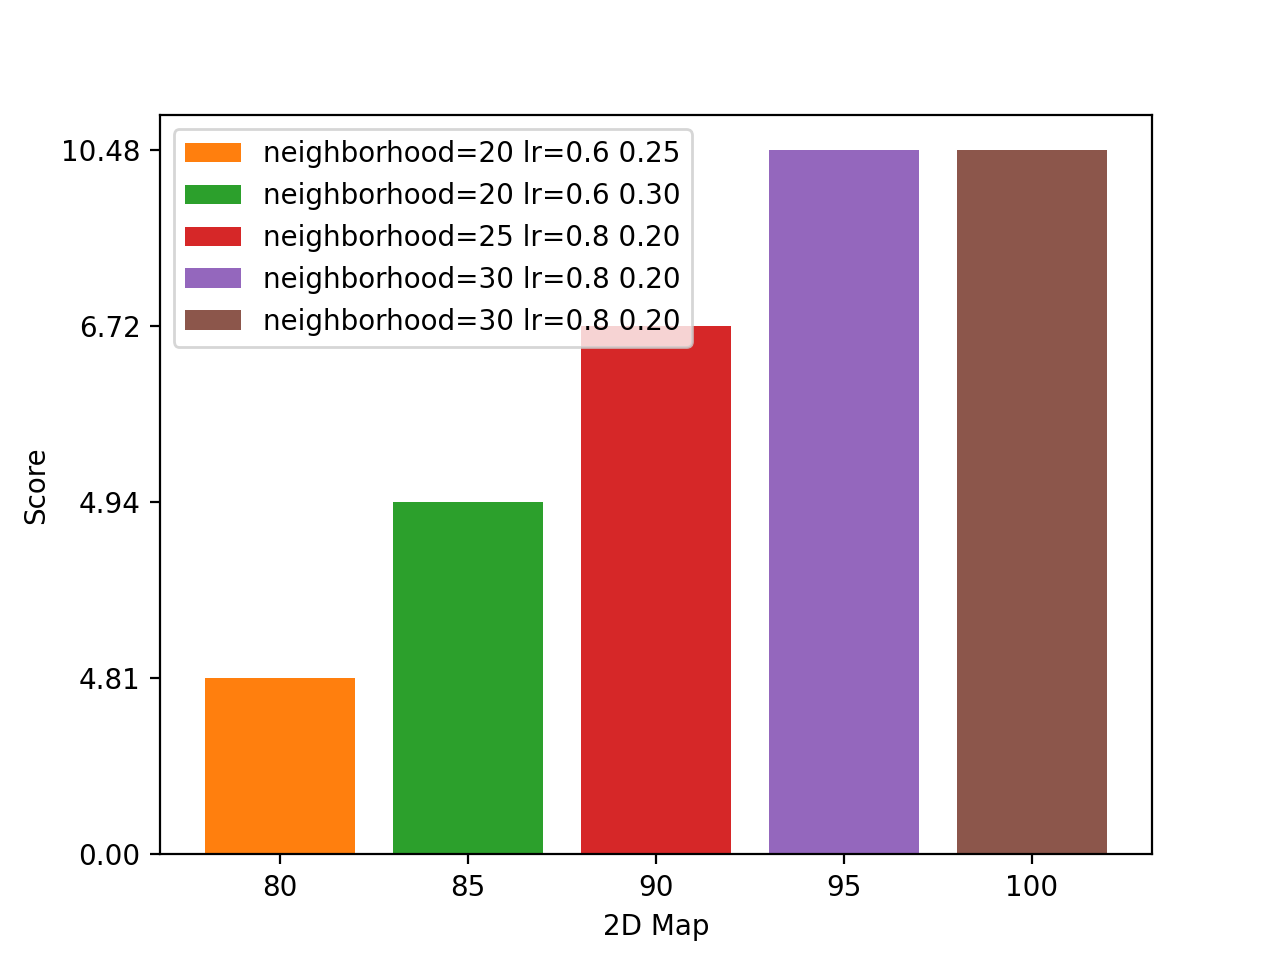
\includegraphics[width=1\textwidth]{Figure_1}
    \caption{Parameter1}
\end{figure}

\begin{figure}[H]
    \centering
    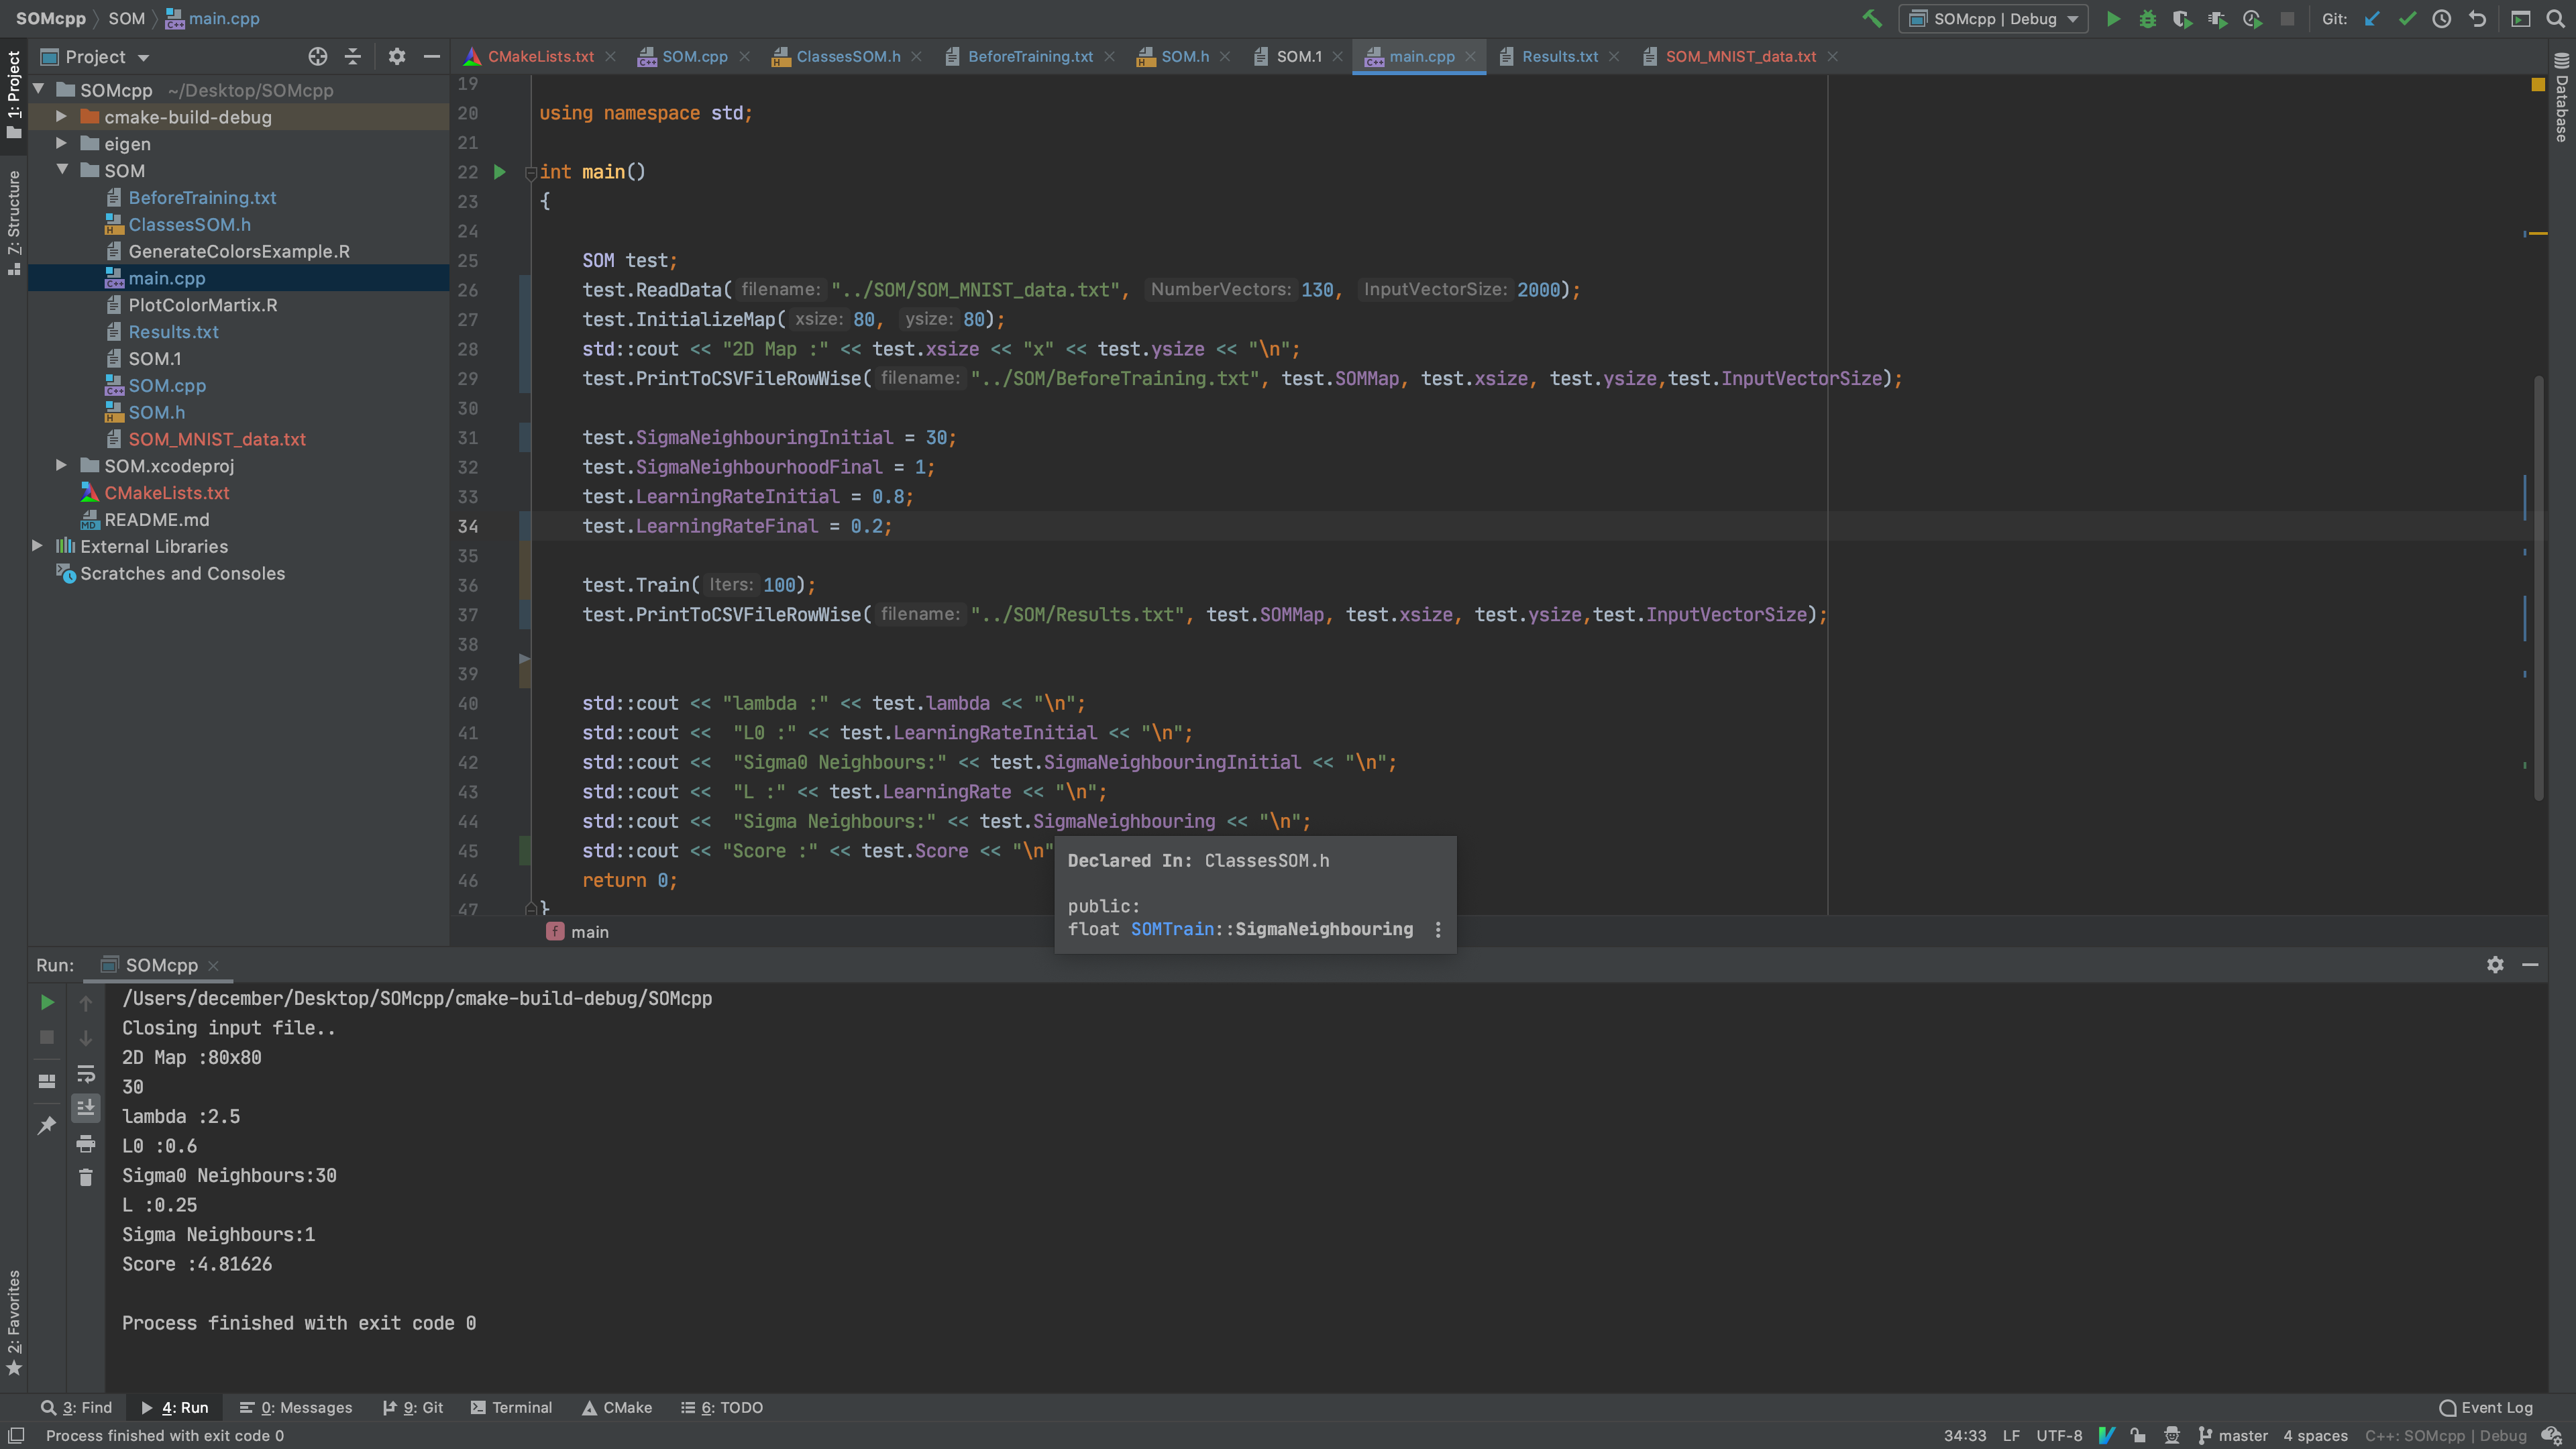
\includegraphics[width=1\textwidth]{Fig1}
    \caption{Parameter1}
\end{figure}

\begin{figure}[H]
    \centering
    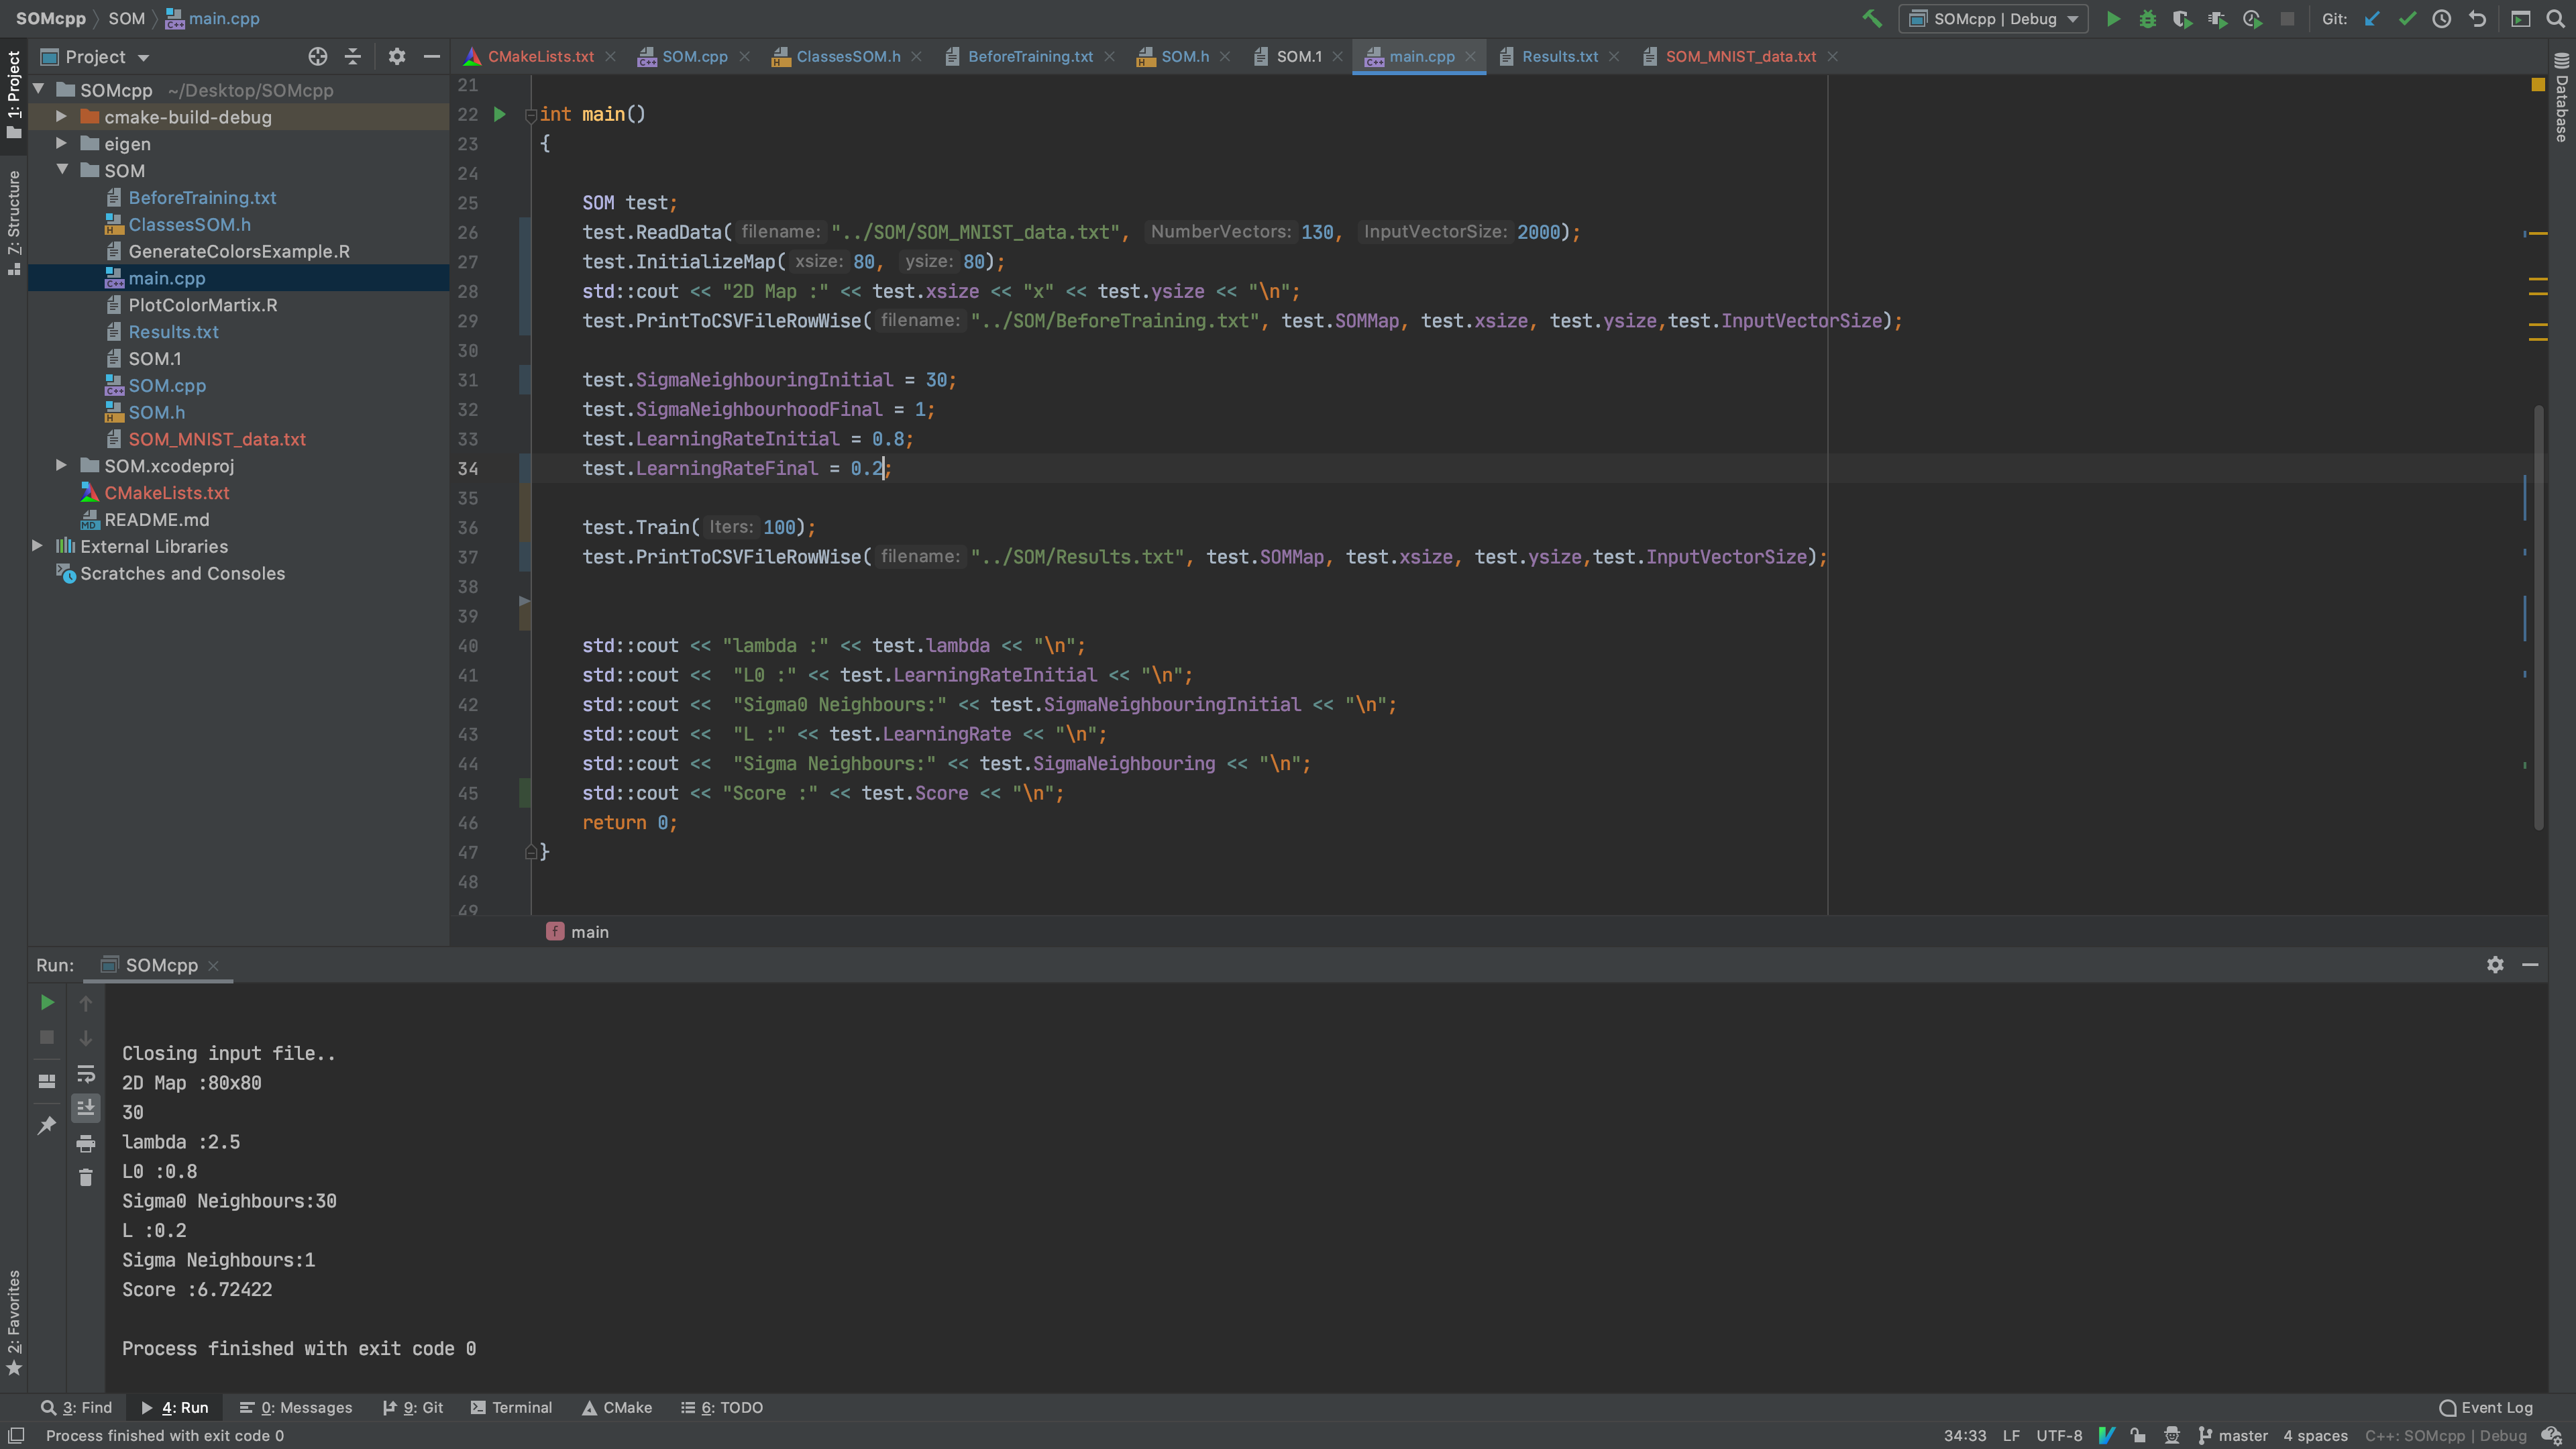
\includegraphics[width=1\textwidth]{Fig2}
    \caption{Parameter2}
\end{figure}


\begin{figure}[H]
    \centering
    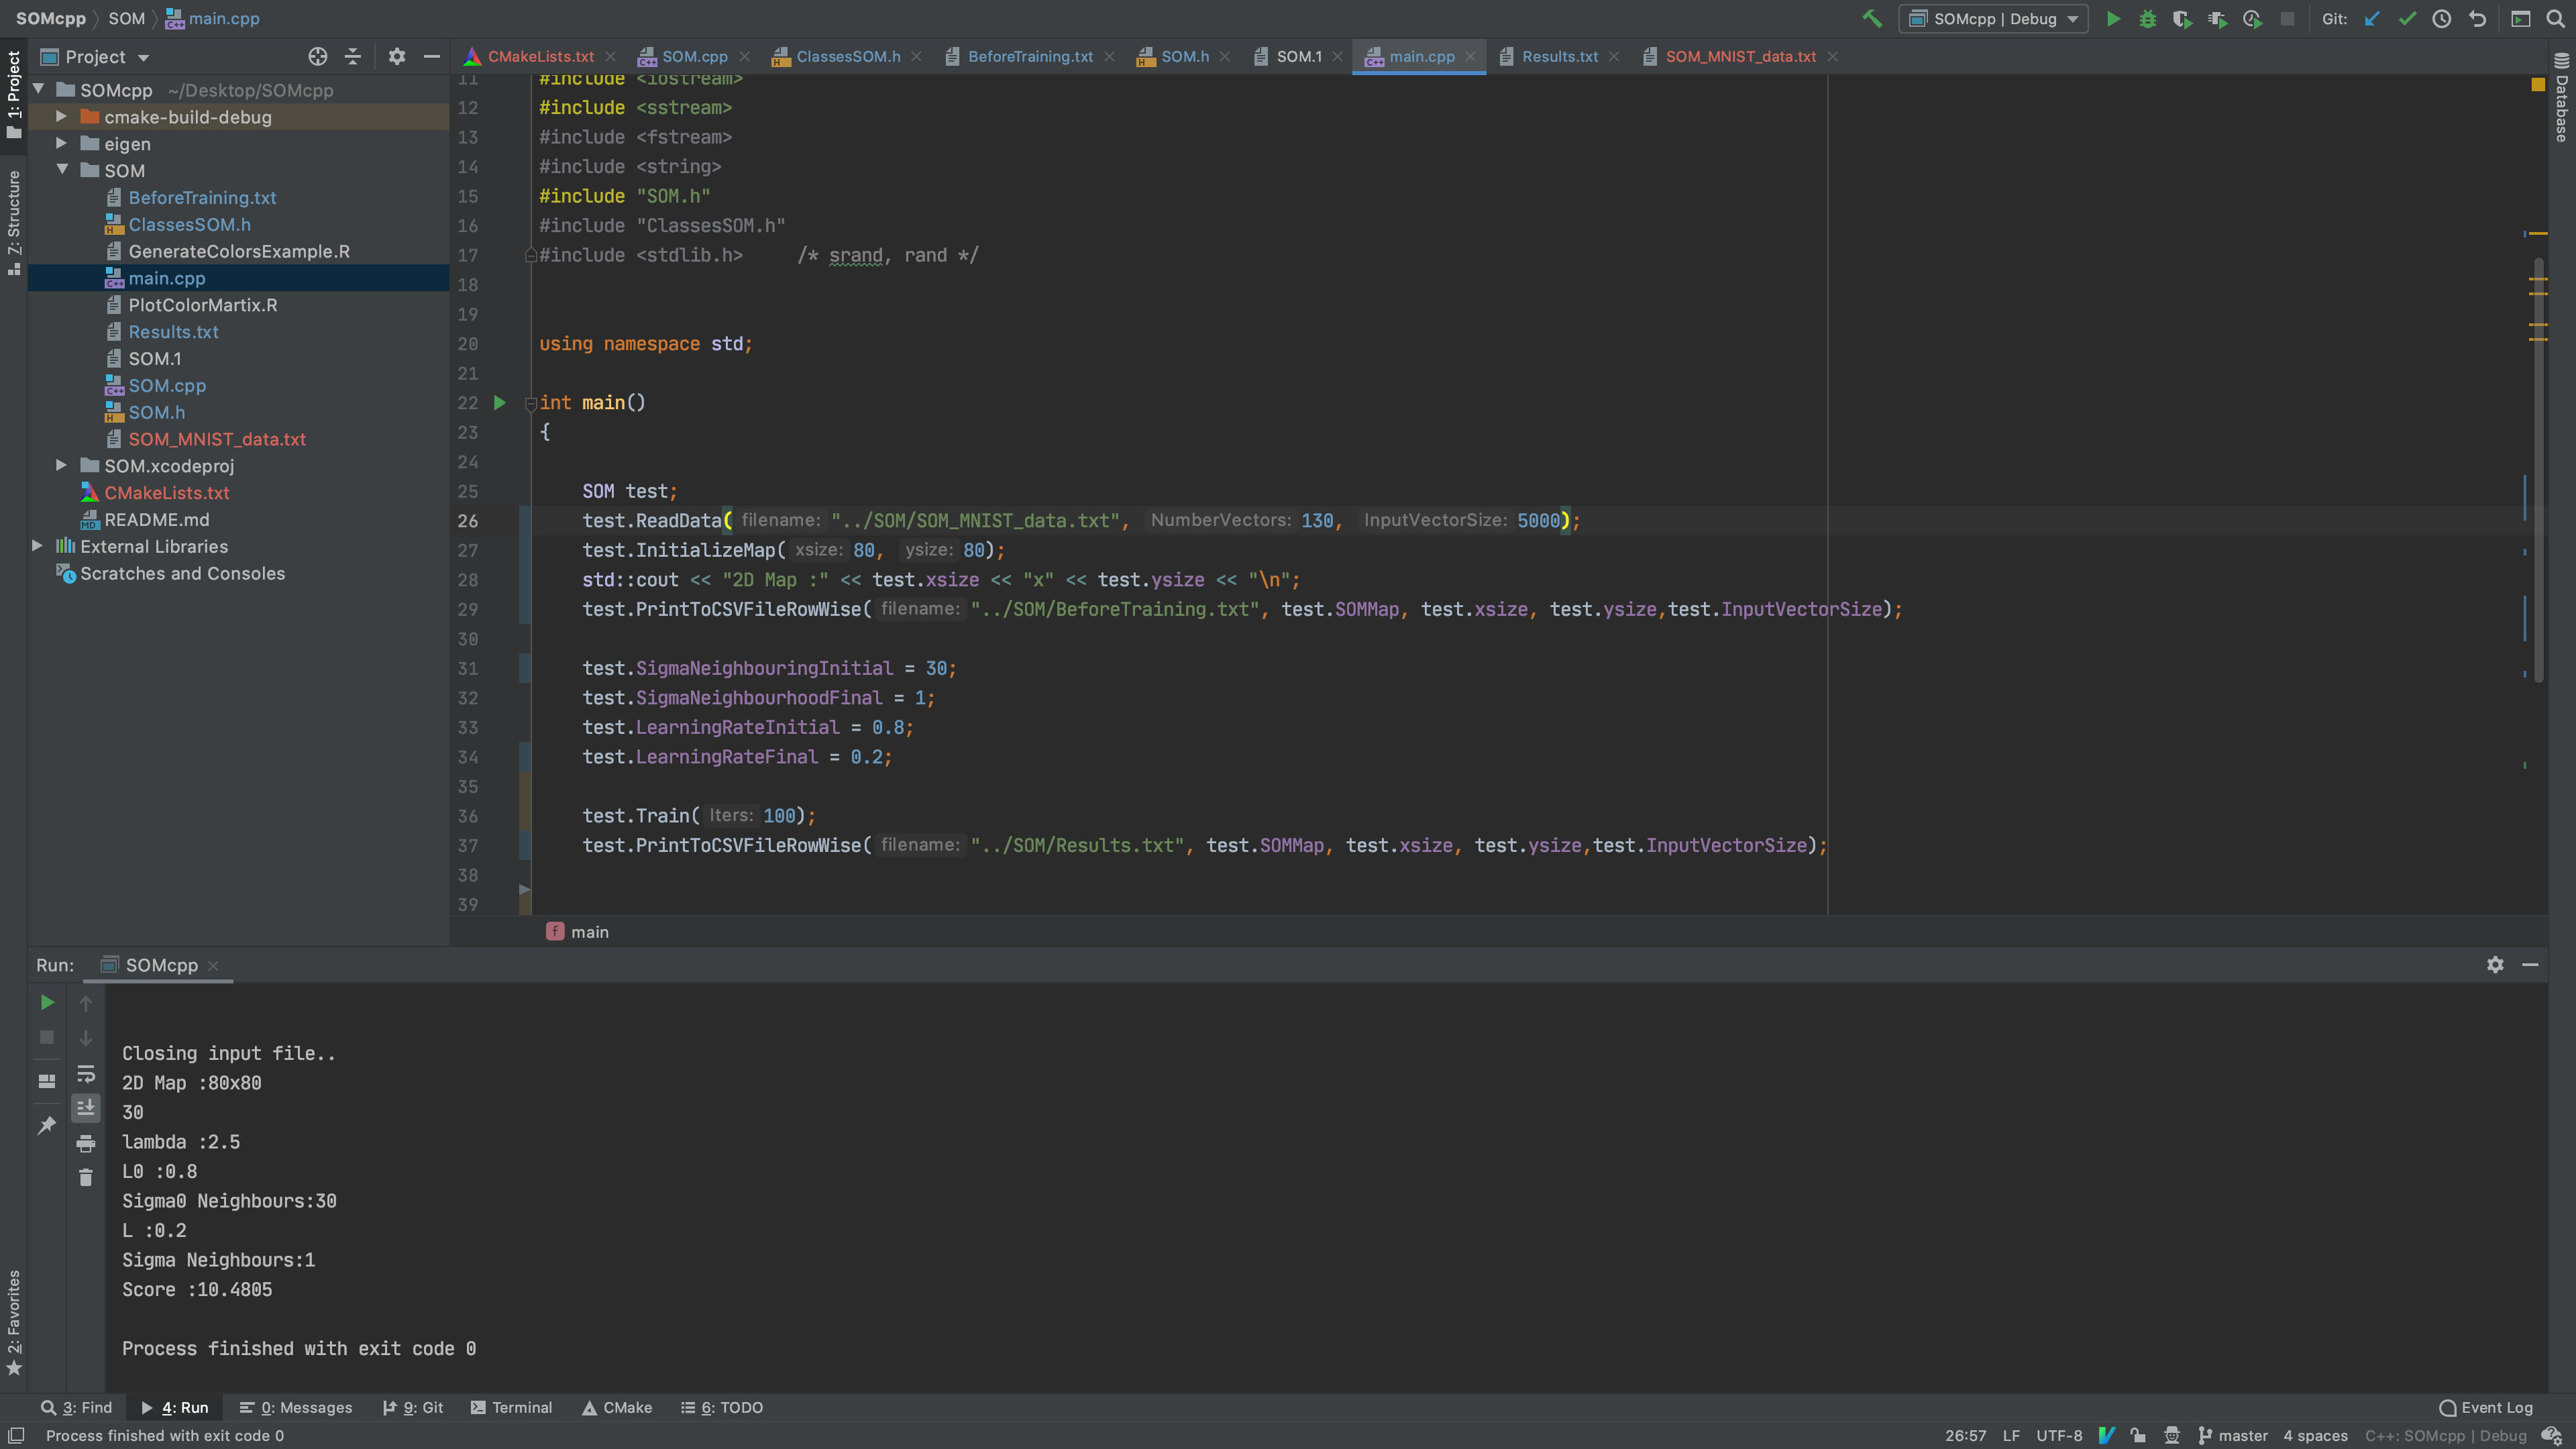
\includegraphics[width=1\textwidth]{Fig3}
    \caption{Parameter3}
\end{figure}


\question{Part1-Step4}{Result}

\begin{figure}[H]
    \centering
    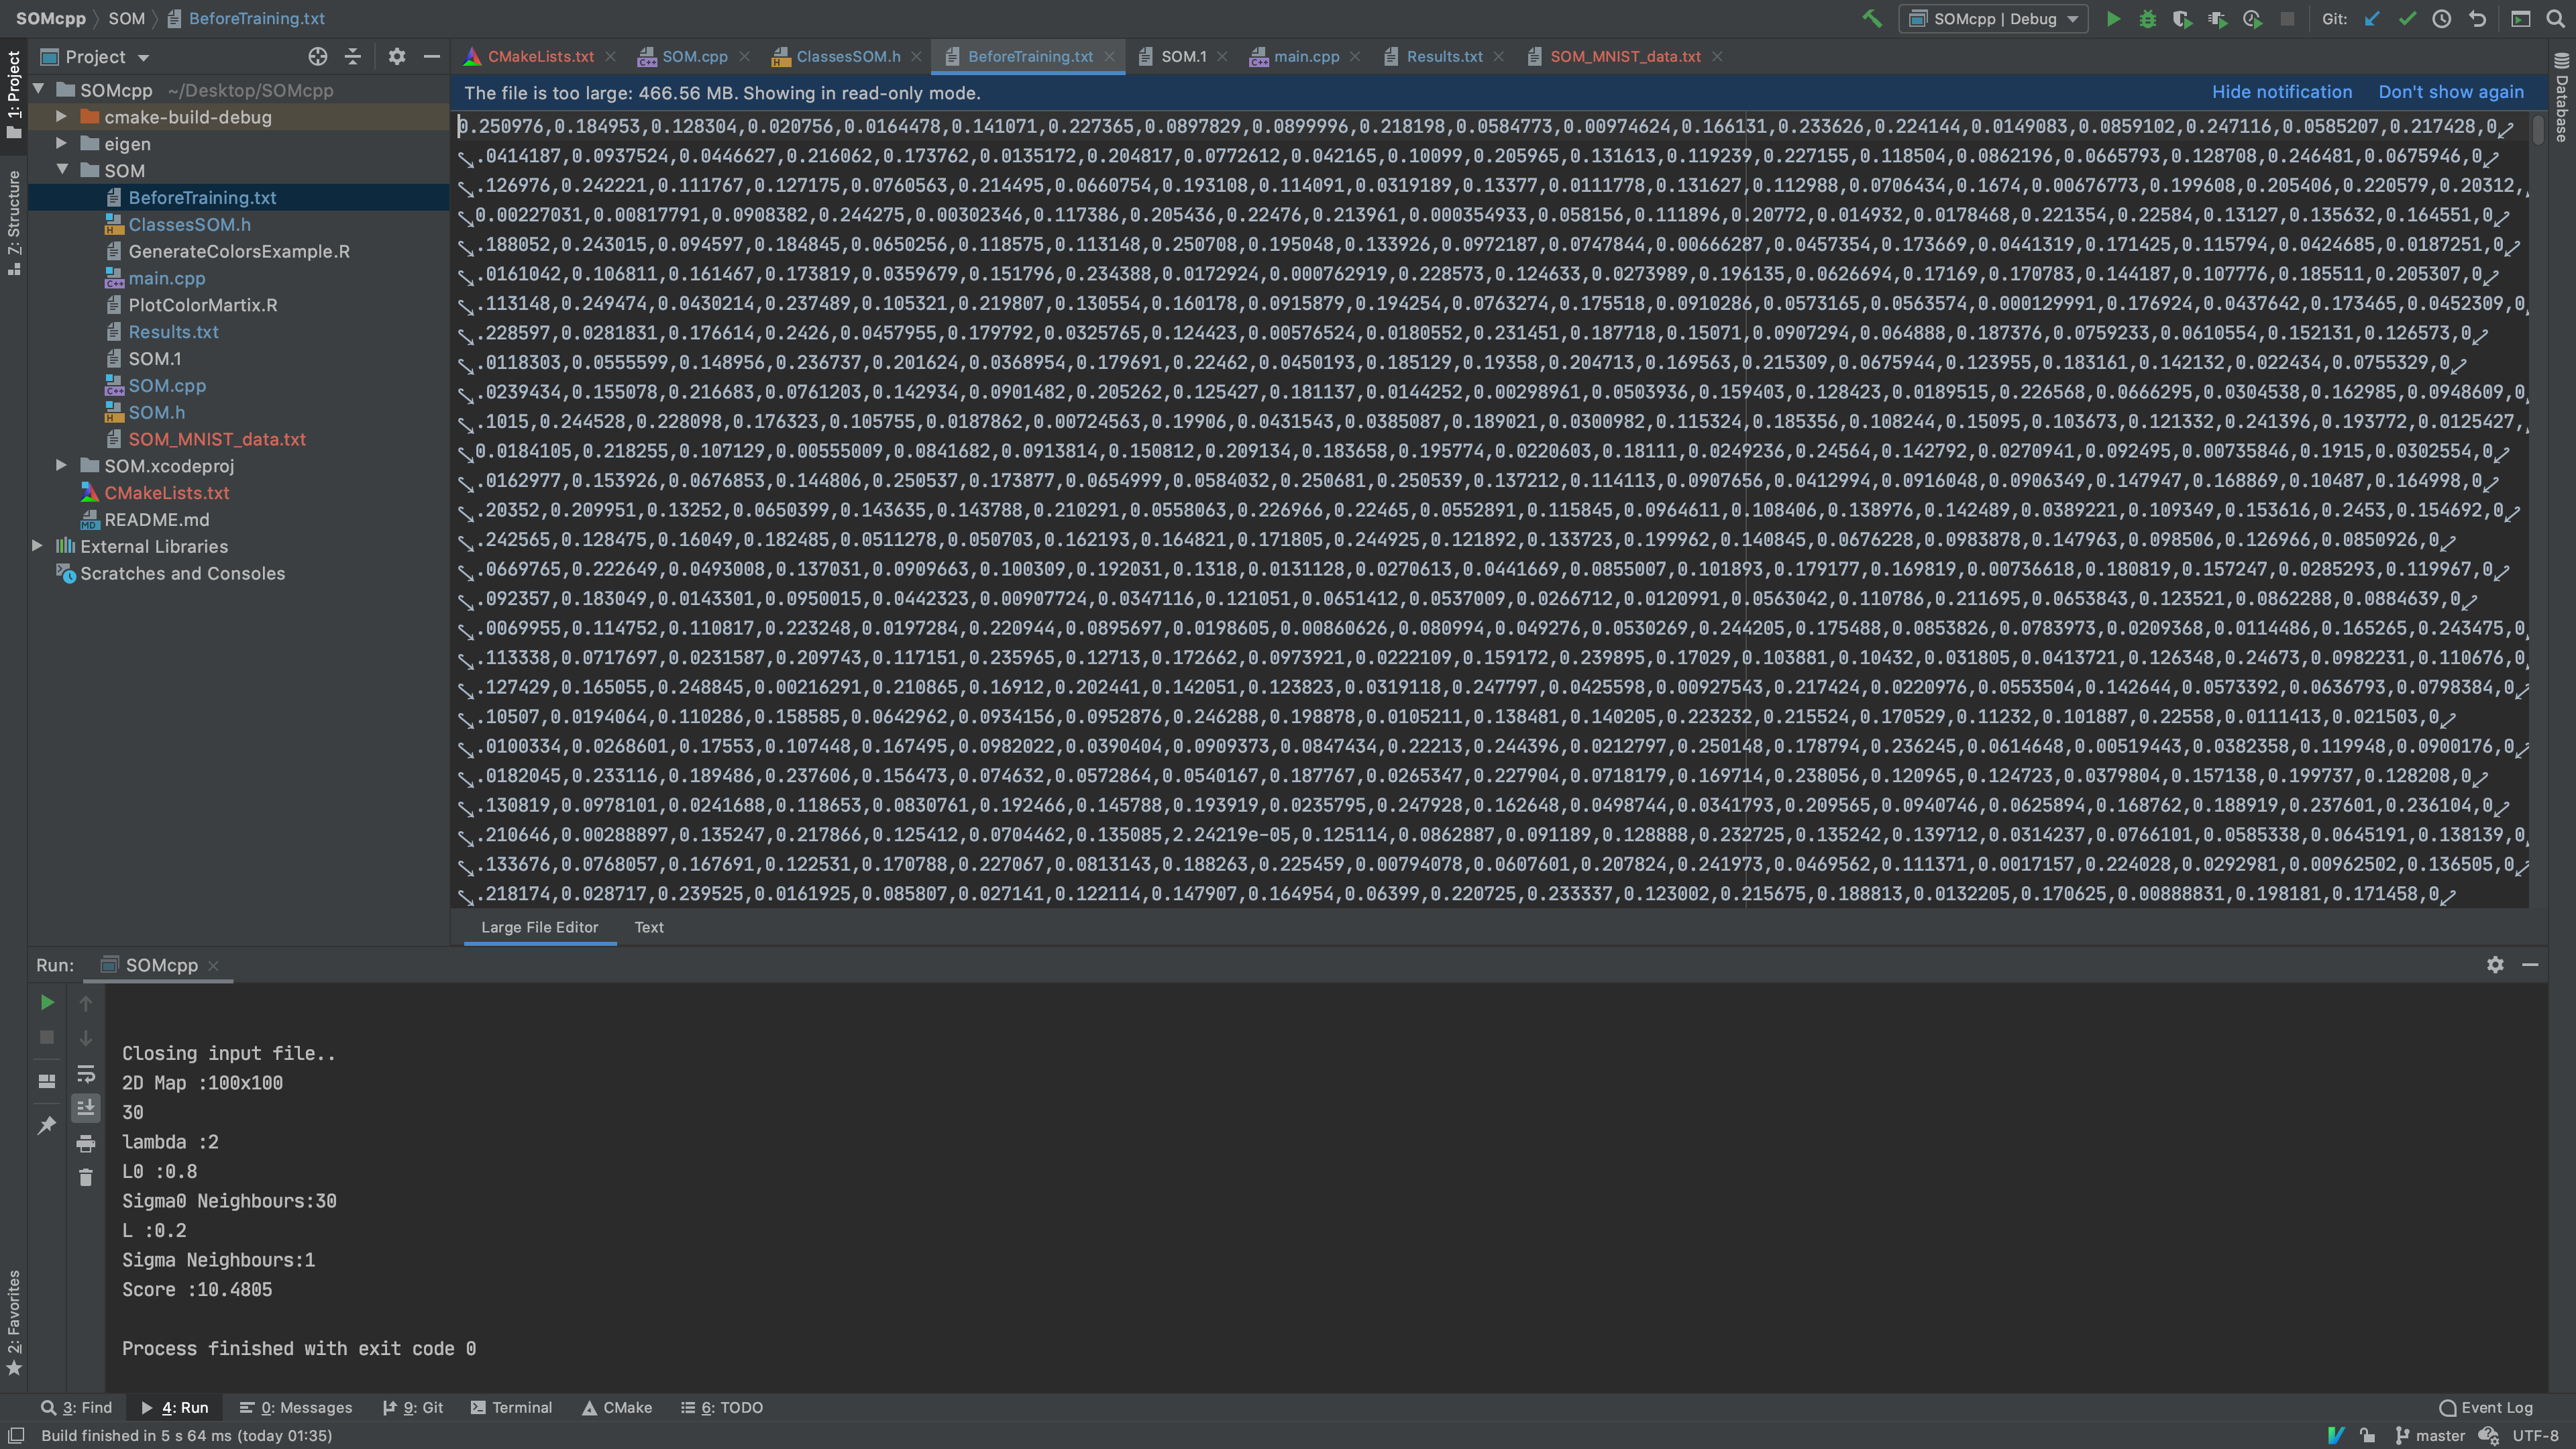
\includegraphics[width=1\textwidth]{Fig5}
    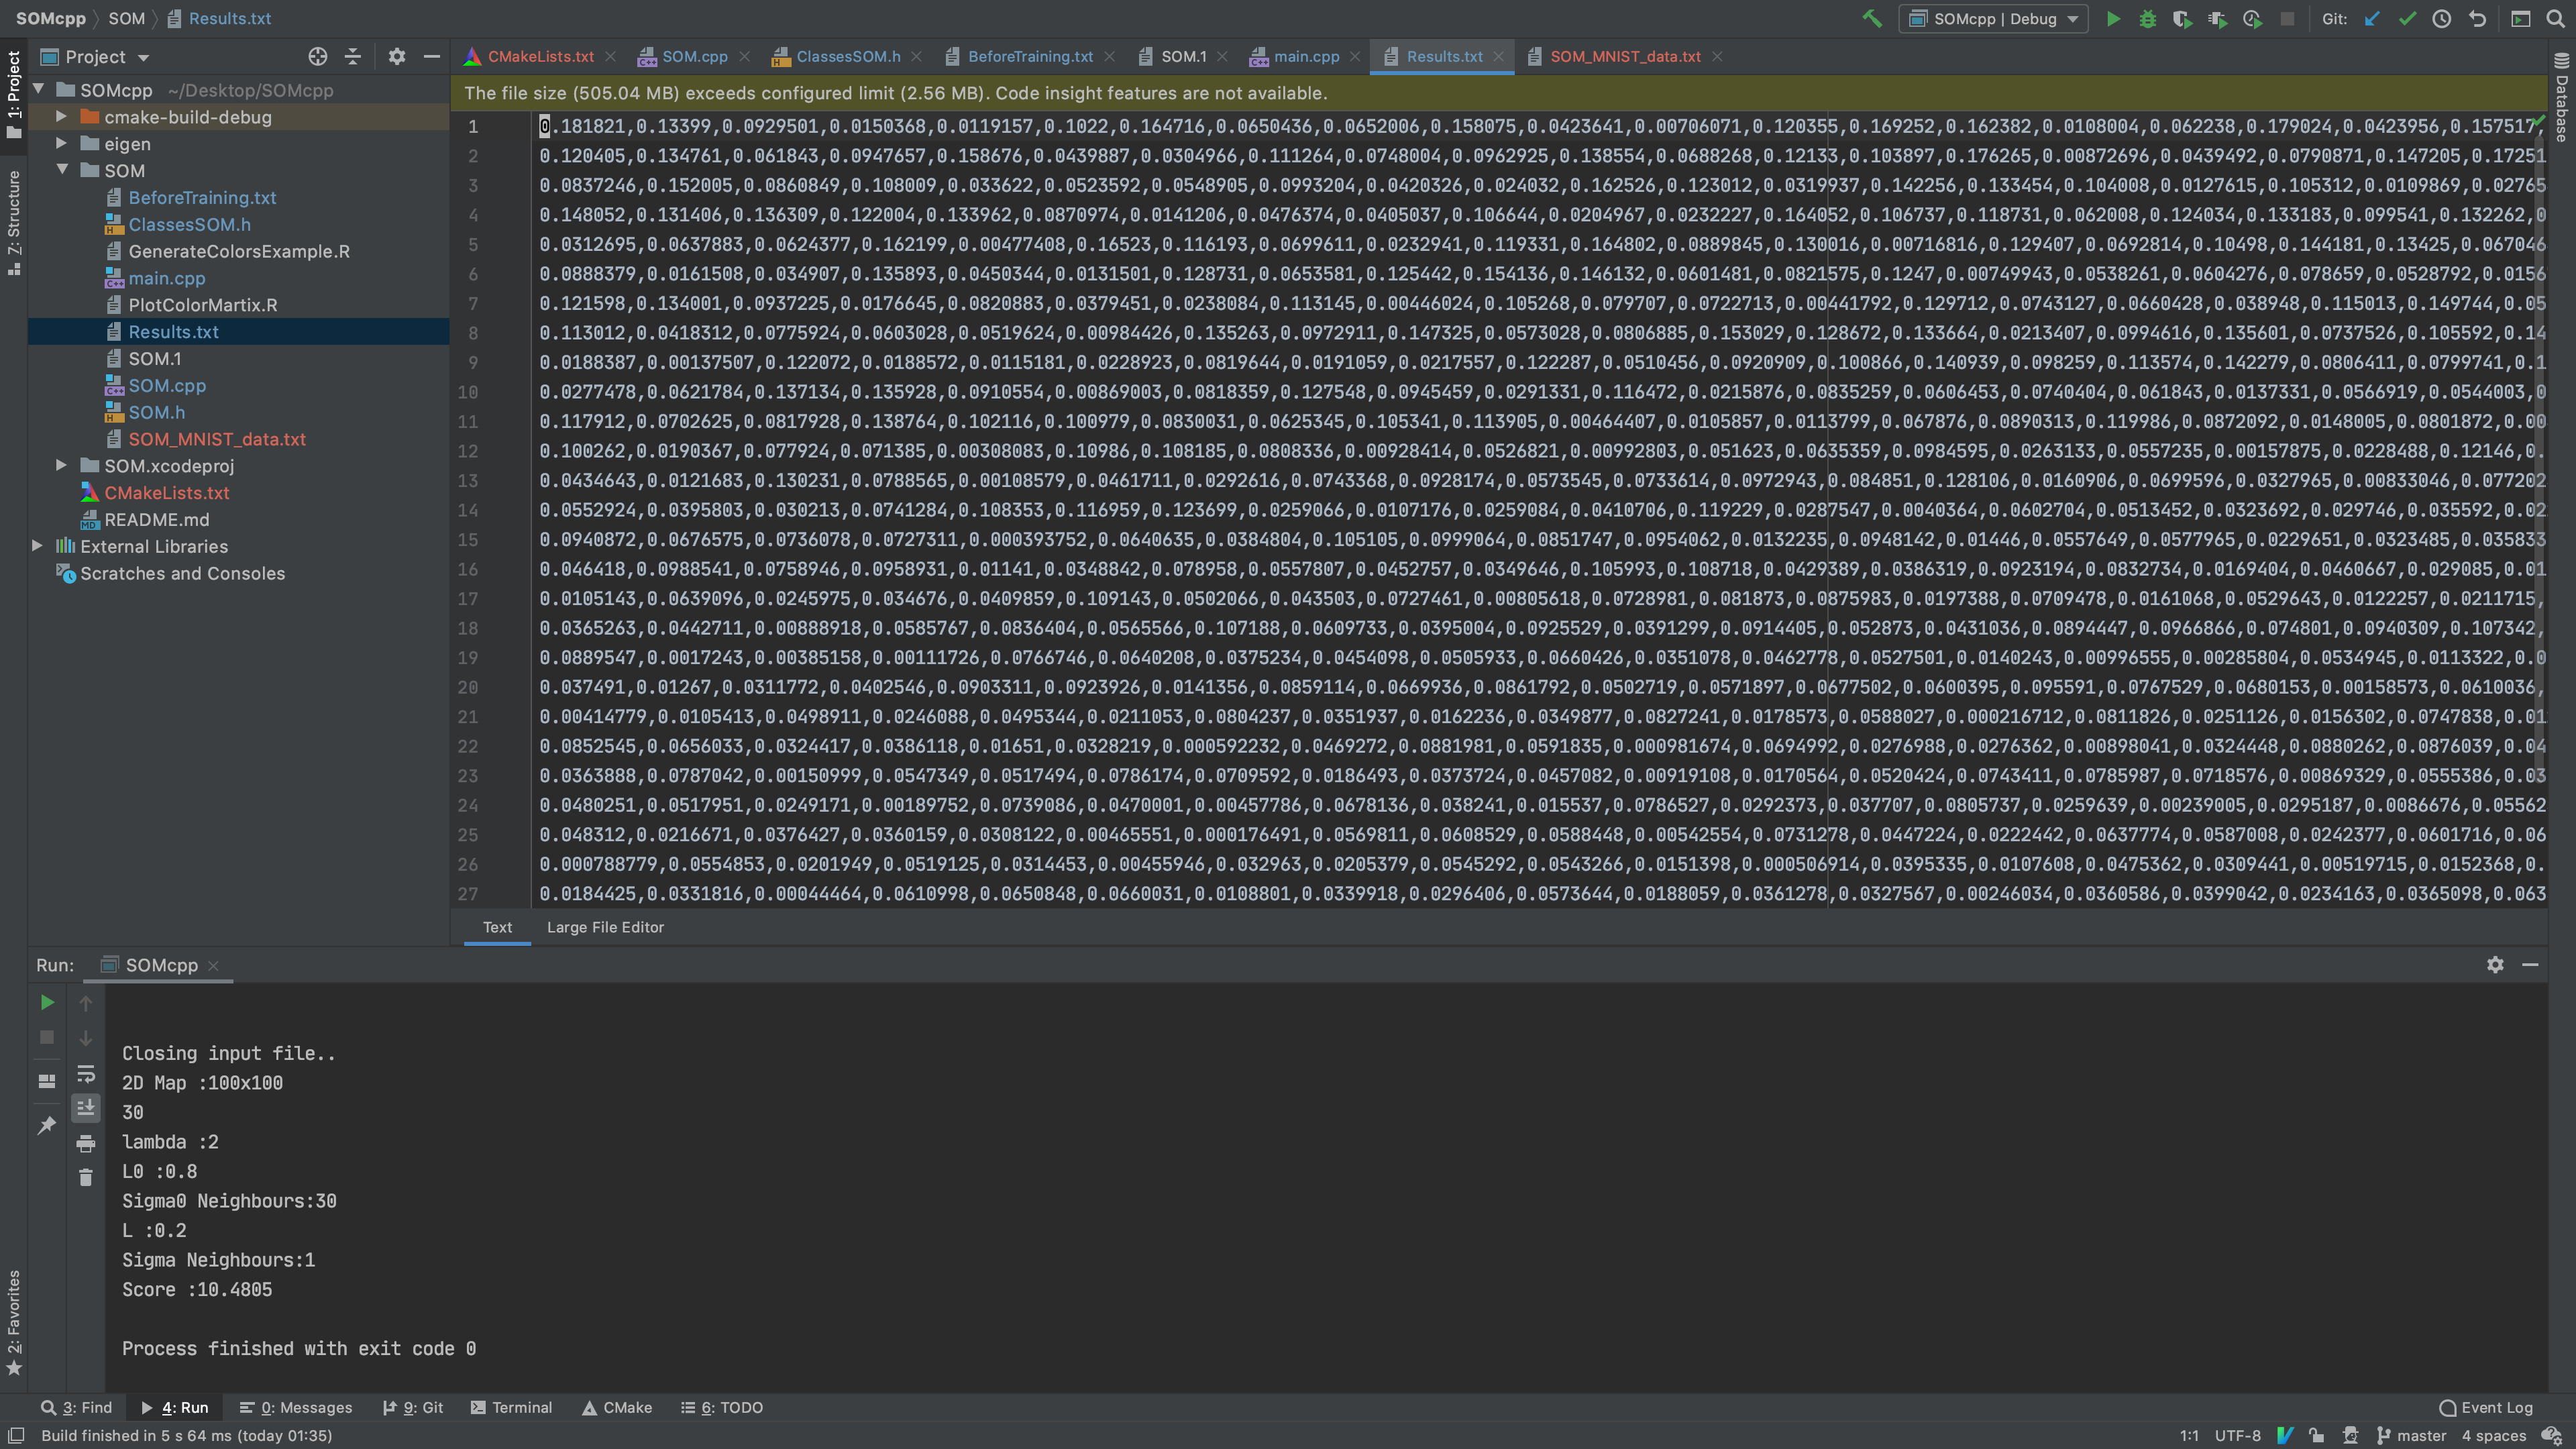
\includegraphics[width=1\textwidth]{Fig4}
    \caption{Output}
\end{figure}


\newpage \question{Part2}{Introduction On MNIST}
The MNIST data is split into three parts: 55,000 data points of training data (mnist.train), 10,000 points of test data (mnist.test), and 5,000 points of validation data (mnist.validation). This split is very important: it's essential in machine learning that we have separate data which we don't learn from so that we can make sure that what we've learned actually generalizes!

the training images are mnist.train.images and the training labels are mnist.train.labels.

Each image is 28 pixels by 28 pixels. Each entry in the tensor is a pixel intensity between 0 and 1, for a particular pixel in a particular image.

Each image in MNIST has a corresponding label, a number between 0 and 9 representing the digit drawn in the image.

\question{Part2}{Multinomial Logistic Regression}
\begin{lstlisting}
learning_rate = 0.09
training_epochs = 20
batch_size = 80
display_step = 1

# mnist data image of shape 28*28=784
# 0 - 9 recognition -> 10 classes
x = tf.placeholder(tf.float32, [None, 784]) 
y = tf.placeholder(tf.float32, [None, 10])


W = tf.Variable(tf.zeros([784, 10]))
b = tf.Variable(tf.zeros([10]))

# softmax model
pred = tf.nn.softmax(tf.matmul(x, W) + b) 

# using cross entropy
# use gradient descent
cost = tf.reduce_mean(-tf.reduce_sum(y*tf.log(pred), reduction_indices=1))
optimizer = tf.train.GradientDescentOptimizer(learning_rate).minimize(cost)
\end{lstlisting}


\begin{figure}[H]
    \centering
    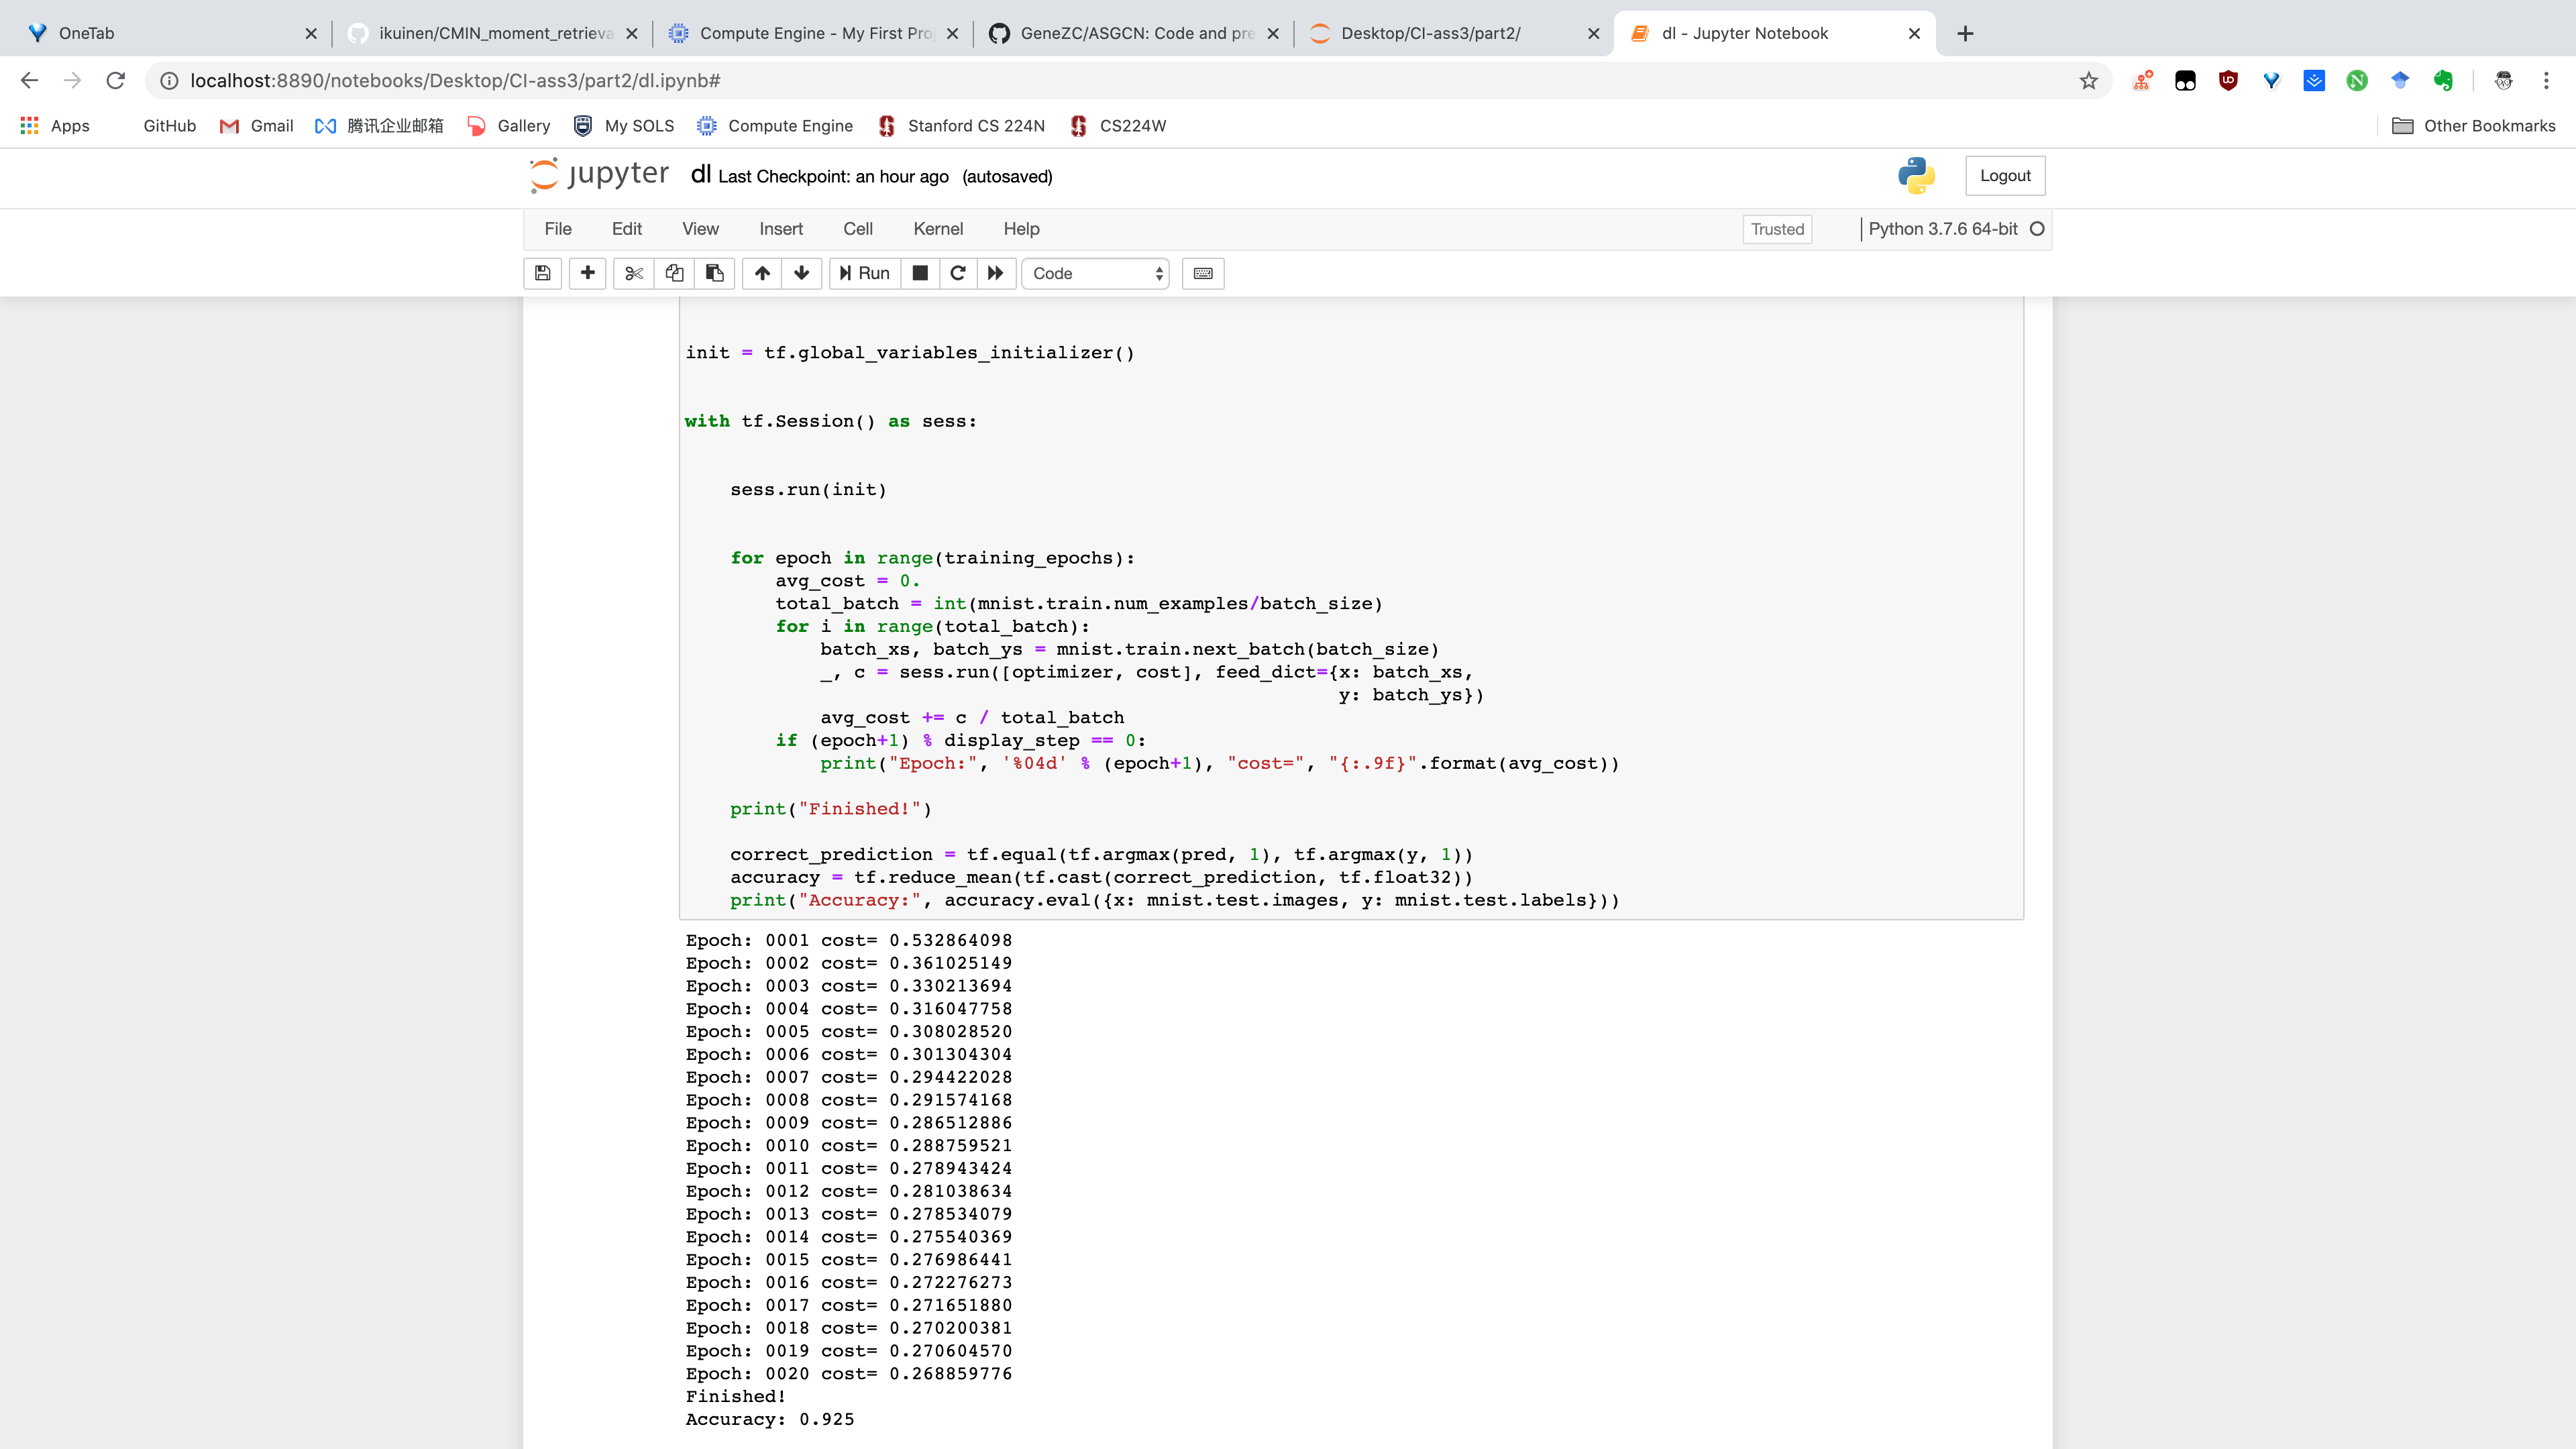
\includegraphics[width=1\textwidth]{Fig6}
    \caption{Multinomial Logistic Regression Output}
\end{figure}

\question{Part2}{CNN}

\begin{lstlisting}
learning_rate = 0.009
num_steps = 2000
batch_size = 128

num_input = 784 
num_classes = 10 
dropout = 0.25


# Create the neural network
def conv_net(x_dict, n_classes, dropout, reuse, is_training):
    with tf.variable_scope('ConvNet', reuse=reuse):
        x = x_dict['images']

        x = tf.reshape(x, shape=[-1, 28, 28, 1])

        # 32 filters and 5 kernels in Convolution Layer
        conv1 = tf.layers.conv2d(x, 32, 5, activation=tf.nn.relu)
        conv1 = tf.layers.max_pooling2d(conv1, 2, 2)

        # 64 filters and 3 kernels in Convolution Layer2
        conv2 = tf.layers.conv2d(conv1, 64, 3, activation=tf.nn.relu)
        conv2 = tf.layers.max_pooling2d(conv2, 2, 2)

        fc1 = tf.contrib.layers.flatten(conv2)

        fc1 = tf.layers.dense(fc1, 1024)
        fc1 = tf.layers.dropout(fc1, rate=dropout, training=is_training)

        out = tf.layers.dense(fc1, n_classes)

    return out
\end{lstlisting}


\begin{figure}[H]
    \centering
    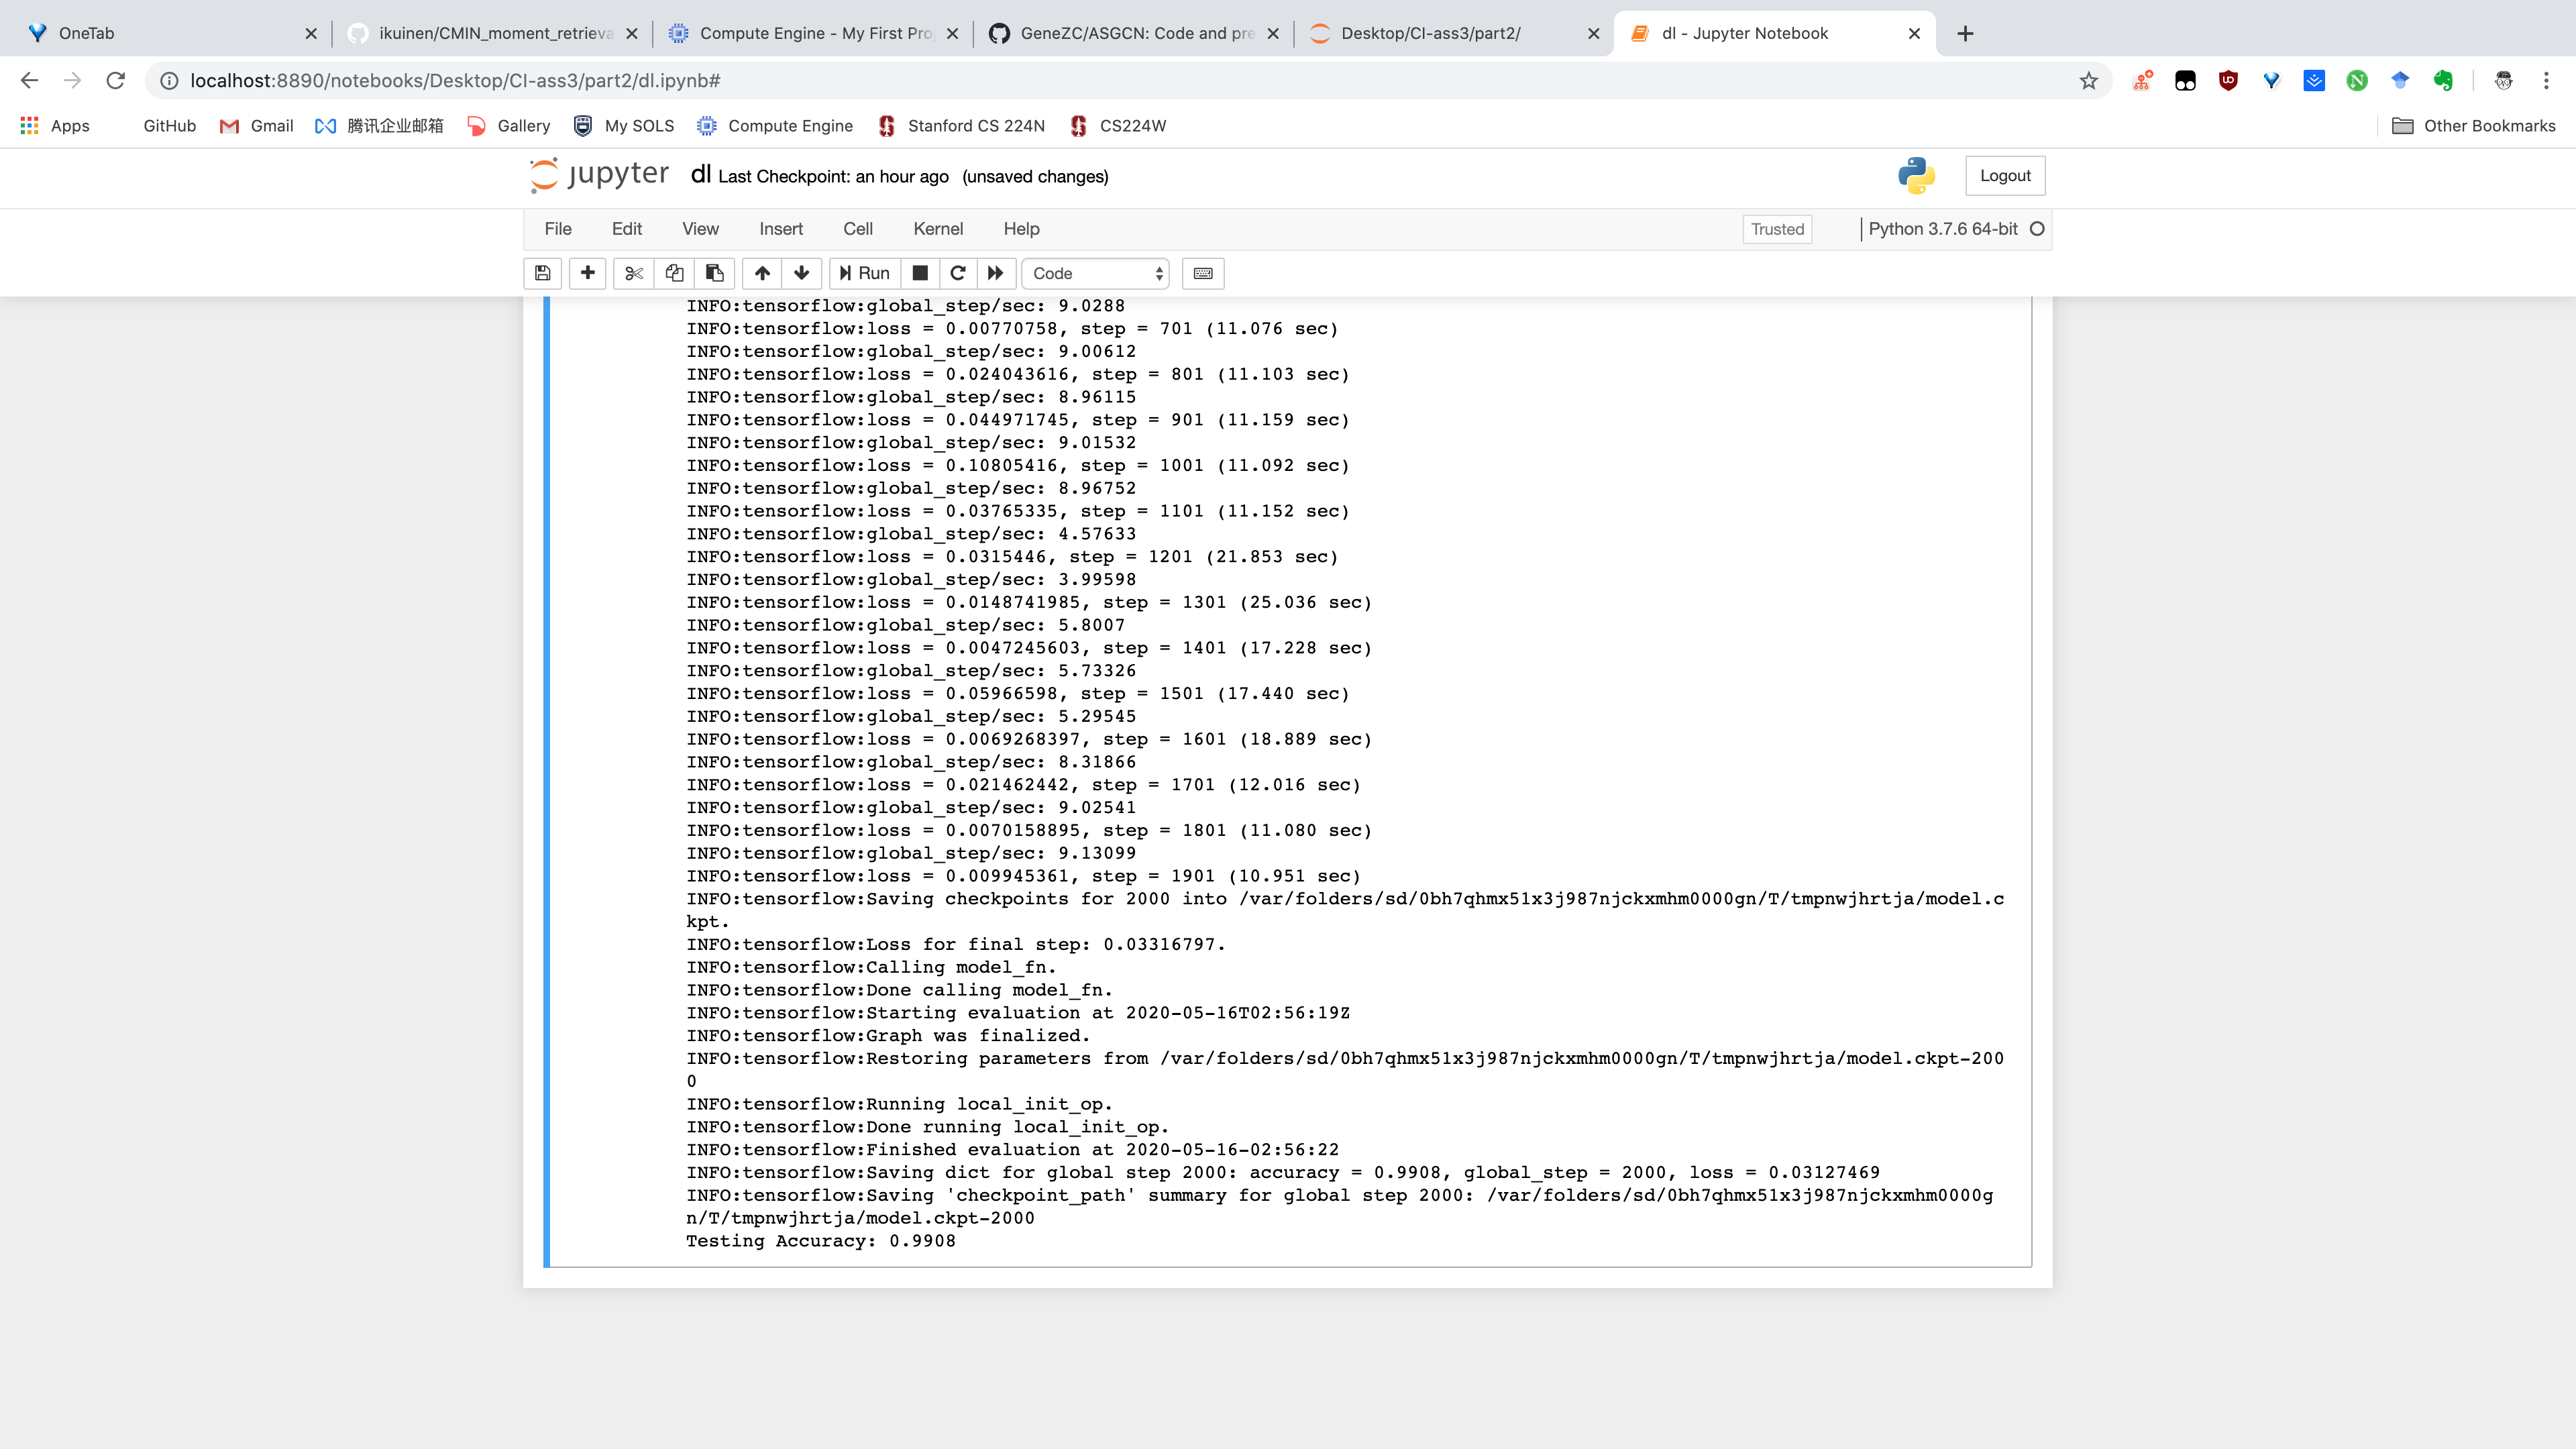
\includegraphics[width=1\textwidth]{Fig7}
    \caption{CNN Output}
\end{figure}


\question{Part2}{Cell Image Classification}
\begin{lstlisting}
training_set_size = 25998
test_set_size = 1560

model = keras.Sequential([
    keras.layers.Convolution2D(5,(3,3),input_shape=(img_size,img_size,training_set[0][0].shape[3]),padding='same',data_format='channels_last',activation='relu'),
    keras.layers.MaxPooling2D((2, 2), padding='same'),
    keras.layers.Convolution2D(10,(3,3),padding='same',data_format='channels_last',activation='relu'),
    keras.layers.MaxPooling2D((2, 2), padding='same'),
    keras.layers.Flatten(),
    #keras.layers.Dense(10, activation = 'relu'), # if you have a good CPU/GPU :S
    keras.layers.Dense(1, activation = 'sigmoid')
])

model.compile(optimizer=tf.train.AdamOptimizer(), 
              loss='binary_crossentropy',
              metrics=['accuracy'])

model.summary()

epochs = 10

model.fit_generator(training_set,
                    steps_per_epoch = (training_set_size/batch_size),
                    epochs = epochs,
                    validation_data = test_set,
                    validation_steps = (test_set_size/batch_size))
\end{lstlisting}

\end{document}